\chapter{Redes Wi-Fi}
\label{cap:redes-wifi}

\section{Introdução}
\label{sec:introducao}

Ao longo dos anos, a evolução  dos sistemas e serviços de telecomunicações criou uma necessidade para seus usuários de estarem conectados ``todo tempo'' e ``em qualquer lugar'', isto é, esses usuários desejam estar permanentemente \textit{online}. Para esses usuários, os meios guiados (par trançado, cabo coaxial e fibra óptica) não têm a menor utilidade, pois uma característica essencial para cumprimento destas necessidades é a mobilidade.

No período em que as LANs cabeadas dominavam a infraestrutura de rede de computadores, somente era possível conectar computadores à Internet e entre si por meio de cabos padrão Ethernet. Este tipo de conexão é bastante popular, mas conta com algumas limitações, por exemplo: só se pode movimentar o computador até o limite de alcance do cabo; ambientes com um grande número de computadores podem exigir adaptações na estrutura do prédio para a passagem dos fios; em uma residência, pode ser necessário realizar perfurações na parede para que os cabos alcancem outros cômodos; a manipulação constante ou incorreta pode fazer com que o conector do cabo de rede se danifique \cite{alecrim2008site}.

Usuários móveis precisam transferir dados para seus dispositivos sem depender da infraestrutura de comunicação cabeada tradicional \cite{tanenbaum2011}. A resposta para esses usuários está na comunicação sem fios. Dentro das comunicações \textit{wireless}, as LANs sem fio oferecem uma alternativa bastante interessante como meio de acesso à Internet.

As LANs sem fio são muito populares atualmente, especialmente nas residências, escritórios, instituições acadêmicas e outros lugares onde a instalação de cabos é muito trabalhosa ou inviável física e/ou financeiramente. Embora muitas tecnologias e padrões para LANs sem fio tenham sido desenvolvidos na década de 1990, uma classe particular de padrões surgiu claramente como a vencedora: a LAN sem fio IEEE (IEEE, do inglês, \textit{Institute of Eletrical and Eletronics Engineers}) 802.11, também conhecida como Wi-Fi \cite{kurose2013}.

Wi-Fi, acrônimo de \textit{Wireless Fidelity}\footnote[3]{Apesar de que a Wi-Fi Alliance nunca ter afirmado tal conclusão.} é o termo comumente usado para tecnologia que é padronizado pelo IEEE sob seus 802 padrões de redes locais. Estritamente falando, ``Wi-Fi'' é o nome da marca comercial dado a produtos que são certificados para serem interoperáveis pela Wi-Fi Alliance\footnote[4]{https://www.wi-fi.org/}, que é uma associação comercial que promove o Wi-Fi e realiza as certificações de equipamentos \cite{gorshe2014ieee}.

O padrão Wi-Fi opera nas faixas de 2.4 GHz e 5 GHz, dentro das faixas livres ISM. De qualquer forma, a desregulamentação do espectro da banda ISM estimulou décadas de inovação e tem sido o principal facilitador do acesso sem fio onipresente atualmente \cite{gorshe2014ieee}.

Outro motivo para a proliferação de implementações Wi-Fi é a facilidade de configuração e compatibilidade com as redes Ethernet com fio que precederam o Wi-Fi \cite{gorshe2014ieee}. No ambiente doméstico, a instalação de redes Wi-Fi tem sido relativamente livre de problemas. Mesmo para aqueles que não são tecnicamente experientes, uma instalação profissional não é cara, e geralmente pode ser fornecida pelo provedor de serviços de Internet local.

\section{Elementos de uma Rede Wi-Fi}
\label{elementos-rede-wifi}

Assim como telefones celulares, televisões e rádios, uma rede Wi-Fi usa ondas de rádio que se propagam ao redor do ponto de acesso para estabelecer a comunicação entre os terminais conectados a ele.

Para que os dados possam ser enviados, o adaptador de rede do cliente os converte em sinal de rádio e os transmite através de uma antena. O ponto de acesso recebe o sinal e o decodifica para então enviá-los para a Internet usando uma conexão Ethernet física com fio padrão \cite{brain2001}.

O processo inverso também funciona, com a ponto de acesso recebendo dados da Internet, convertendo-os em um sinal de rádio e enviando-os ao adaptador sem fio do dispositivo de destino \cite{brain2001}.
Para que uma rede Wi-Fi exista e funcione como descrito anteriormente são necessários alguns componentes que desempenham funções fundamentais, tais como:

\begin{compactitem}
	\item Hospedeiros sem fio: são os dispositivos finais que utilizam os serviços providos pelo ponto de acesso (definido mais adiante). Um hospedeiro sem fio pode ser um \textit{notebook}, um \textit{tablet}, um \textit{smartphone} ou um computador de mesa compatível \cite{kurose2013};
	\item Ponto de acesso (ou estação-base): os pontos de acesso são partes fundamentais da infraestrutura de uma rede sem fio, eles possuem a responsabilidade de coordenar as transmissões dos hospedeiros a eles associadas \cite{kurose2013};
	\item Enlaces sem fio: são responsáveis pela comunicação dos hospedeiros com a ponto de acesso por meio de um enlace de rádio, podem possuir taxas, distância e frequência de transmissão diferentes \cite{kurose2013};
	\item Infraestrutura de rede: cada ponto de acesso está conectada a uma rede maior. Além disso, toda a comunicação é feita entre a ponto de acesso e um hospedeiro sem fio através de um único salto sem fio, ou seja, sem nós intermediários \cite{kurose2013}.
\end{compactitem}

A disposição dos elementos descritos anteriormente pode ser vista na \autoref{fig:elementos-rede}.

\begin{figure}[H]
	\centering
	\Caption{\label{fig:elementos-rede}Elementos de uma rede Wi-Fi padrão.}	
	\UECEfig{}{
		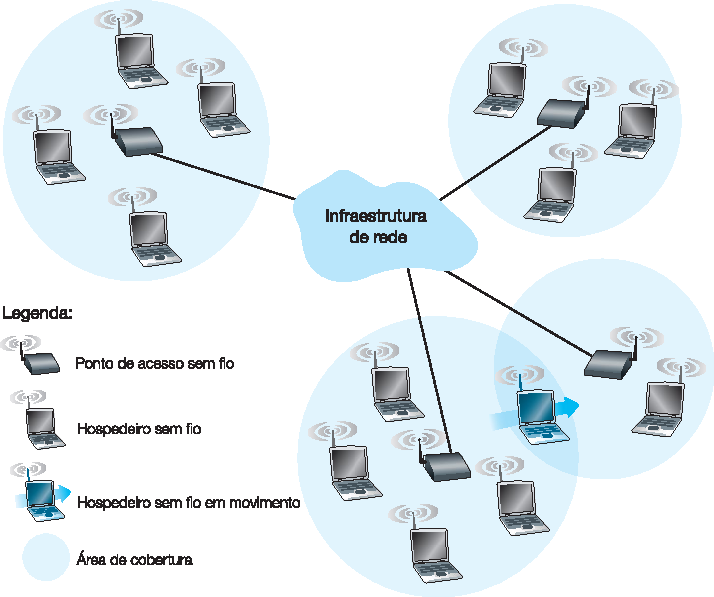
\includegraphics[scale=.77]{figuras/elementos_rede_wireless.pdf}
	}{
		\Fonte{\citeonline[p. ~383]{kurose2013}.}
	}	
\end{figure}

\section{Topologias de LANs sem Fio}
\label{topologias-lans-sem-fio}

As LANs sem fio podem ser estruturadas para operar em dois modos: modo de infraestrutura e modo \textit{ad hoc}.

No modo de infraestrutura, mostrado na \autoref{fig:topologias}(a), cada cliente está associado a um ponto de acesso, que, por sua vez, está conectado a outra rede, geralmente à Internet. O cliente transmite e recebe seus pacotes por meio do ponto de acesso \cite{tanenbaum2011}. Essa topologia é a mais comumente usada, e não é diferente da topologia de uma rede celular.

O outro modo, mostrado na \autoref{fig:topologias}(b), é um exemplo de rede \textit{ad hoc}. Esse modo é um conjunto de terminais móveis que estão interligados de modo que possam enviar dados diretamente uns aos outros. Não existe ponto de acesso nessa configuração, portanto os próprios dispositivos são responsáveis pelo gerenciamento dos recursos da rede. Porém, como o acesso à Internet é a principal aplicação para redes sem fio, as redes \textit{ad hoc} não são muito populares \cite{tanenbaum2011}.

\begin{figure}[H]
	\centering
	\Caption{\label{fig:topologias}Topologias de redes sem fio. (a) Modo de infraestrutura. (b) Modo \textit{ad hoc}.}	
	\UECEfig{}{
		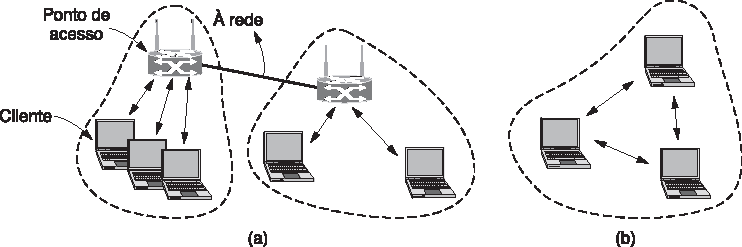
\includegraphics[scale=.9]{figuras/arquiteturas_802-11_tanenbaum.pdf}
	}{
		\Fonte{\citeonline[p. ~188]{tanenbaum2011}.}
	}	
\end{figure}

\section{Arquitetura da LAN sem Fio 802.11}
\label{arquitetura-802-11}

Um sistema de LAN sem fio Wi-Fi geralmente consiste em dois tipos de nós: clientes e pontos de acesso. O ponto de acesso (\autoref{fig:ap}), chamado de roteador sem fio é o ponto central de qualquer rede sem fio. O ponto de acesso conecta todos os equipamentos sem fio à rede tradicional cabeada, onde está a conexão com a Internet.

\begin{figure}[H]
	\centering
	\Caption{\label{fig:ap}Ponto de acesso da fabricante 3Com.}	
	\UECEfig{}{
		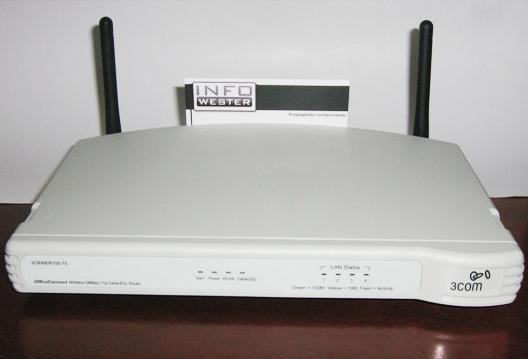
\includegraphics[scale=.62]{figuras/routerwf.jpg}
	}{
		\Fonte{\citeonline{alecrim2008site}.}
	}	
\end{figure}

Os clientes da rede sem fio são os computadores de mesa, \textit{notebooks}, agendas eletrônicas (PDA, do inglês, \textit{Personal Digital Assistant}), \textit{smartphones} e até consoles de videogame (\autoref{fig:clientes}). Para conectarem-se a uma rede sem fio, os equipamentos precisam ter uma interface Wi-Fi. Atualmente, a maioria dos clientes já possui uma placa Wi-Fi integrada de fábrica.

\begin{figure}[H]
	\centering
	\Caption{\label{fig:clientes}Exemplos de clientes sem fio.}	
	\UECEfig{}{
		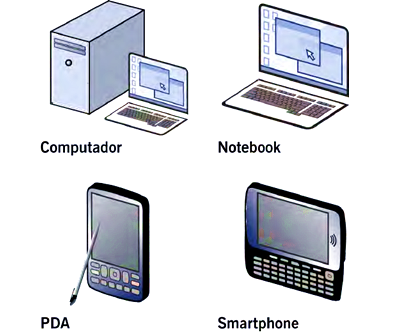
\includegraphics[scale=.75]{figuras/clientes.png}
	}{
		\Fonte{\citeonline[p. ~8]{fluminense2010}.}
	}	
\end{figure}

A \autoref{fig:arquitetura} ilustra os principais elementos da arquitetura de uma LAN sem fio 802.11. O bloco de construção fundamental da arquitetura 802.11 é o Conjunto Básico de Serviço (BSS, do inglês, \textit{Basic Service Set}). Um BSS contém uma ou mais estações sem fio e um ponto de acesso e possui a função de controlar quando cada cliente móvel pode transmitir. O Sistema de Distribuição (DS, do inglês, \textit{Distribution System}) é o local da topologia onde os pontos de acesso se interconectam numa rede cabeada, podendo ser numa rede padrão Ethernet ou num \textit{backbone}. O Ponto de Serviço Estendido (ESS, do inglês, \textit{Extended Service Set}) é o ponto ou um grupo de pontos básicos de serviço interconectados por um sistema de distribuição \cite{moraes2010}.

\begin{figure}[H]
	\centering
	\Caption{\label{fig:arquitetura}Arquitetura típica de uma LAN IEEE 802.11.}	
	\UECEfig{}{
		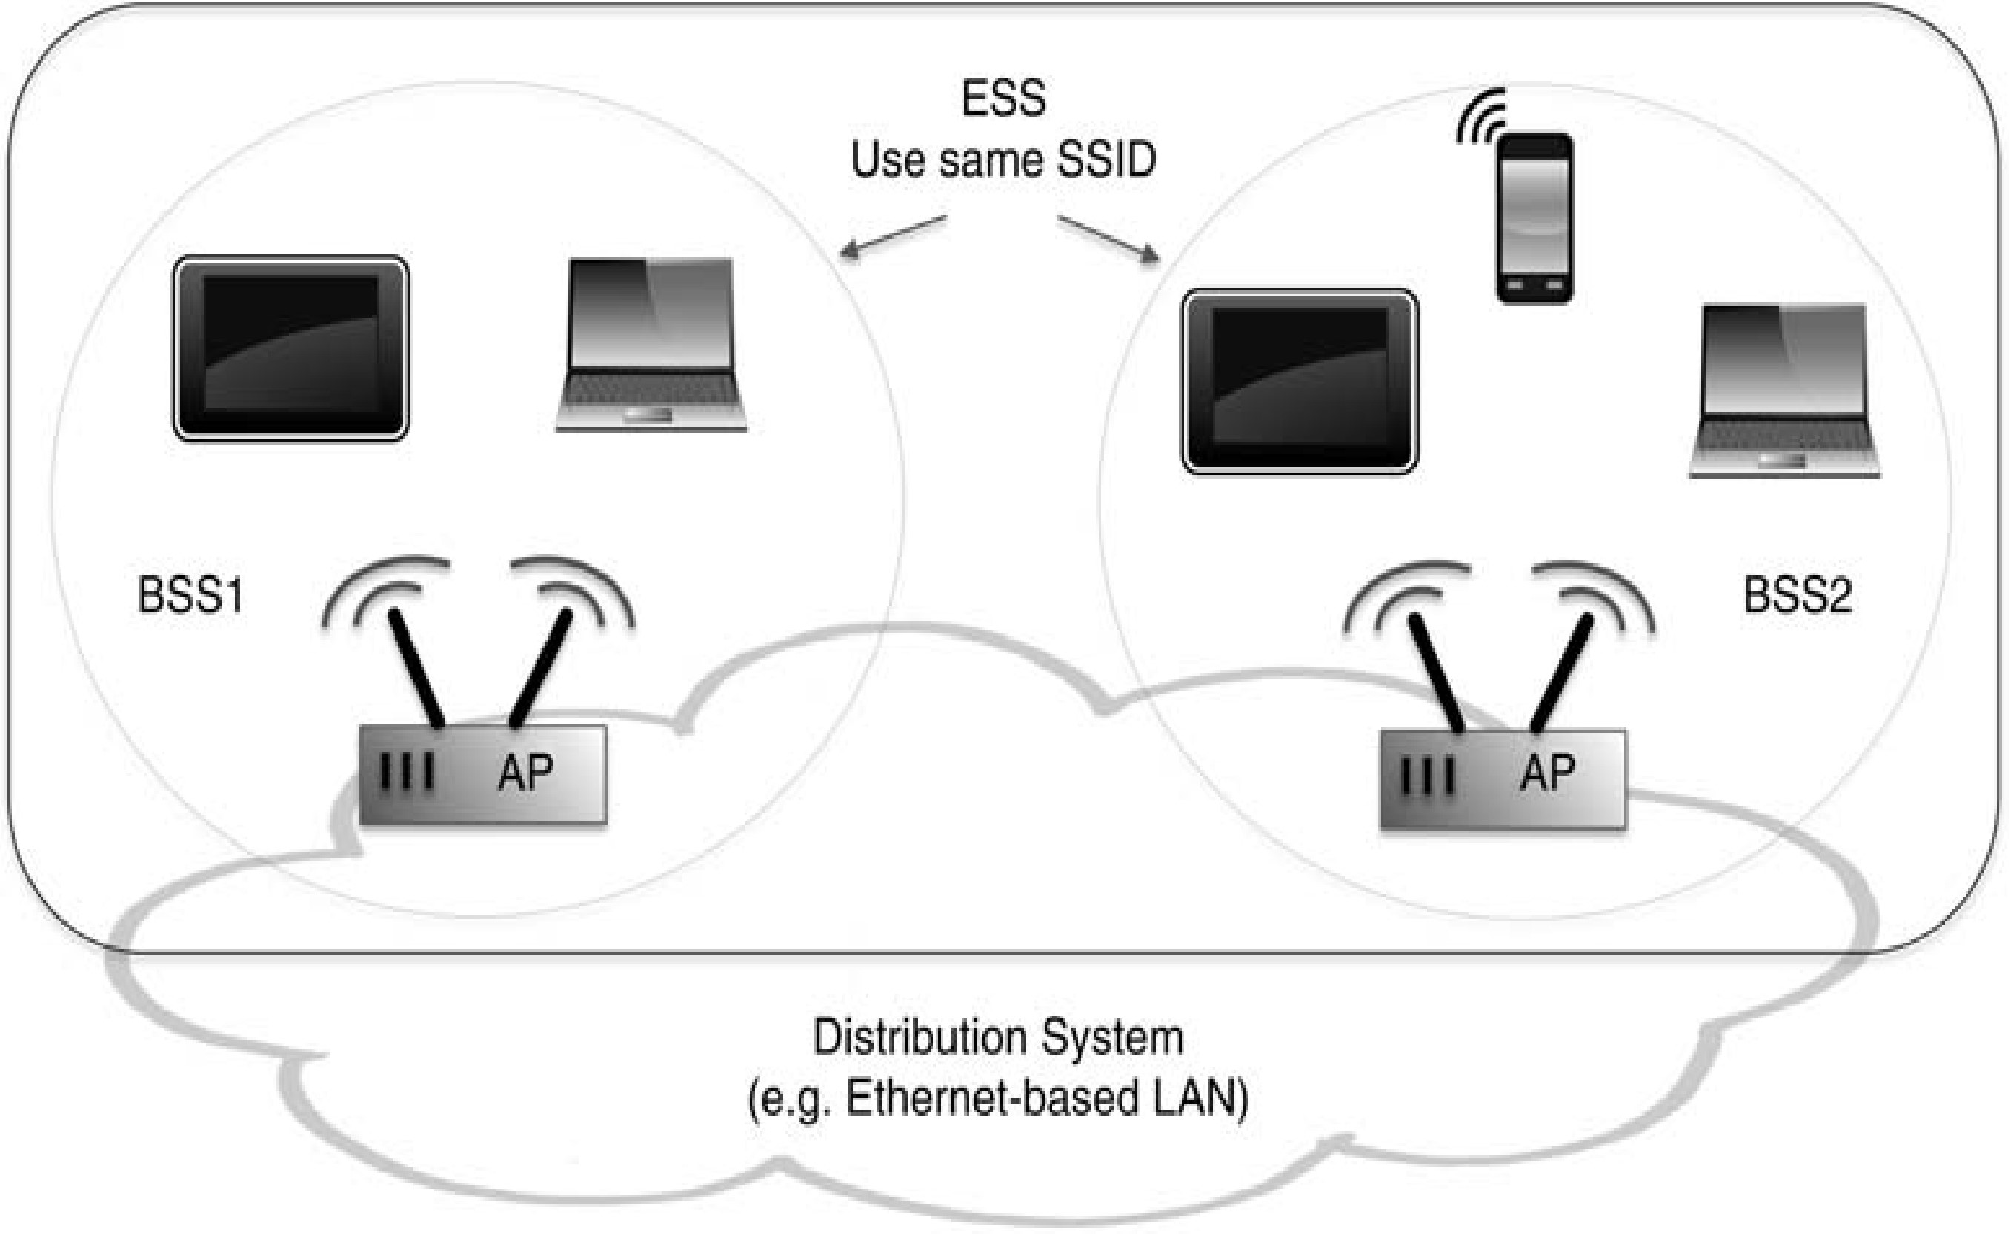
\includegraphics[scale=.33]{figuras/arquiteturas_802-11_01.pdf}
	}{
		\Fonte{\citeonline[p. ~308]{gorshe2014ieee}.}
	}	
\end{figure}

Outro ponto importante na arquitetura 802.11 consiste no fato de a rede permitir a mudança automática e transparente para o usuário quando este sai de sua célula (BSS) e vai para outra célula vizinha, processo este conhecido como \textit{roaming}. Cada célula contém o seu ponto de acesso e por esse motivo o \textit{roaming} multicanal oferece maior abrangência e mobilidade ao sistema (MORAES, 2014).

\subsection{Canais}
\label{subsec:canais}

Como pode ser visto na \autoref{fig:ism_unii}, a faixa de frequência de 2.4 GHz aloca 83,5 MHz do espectro eletromagnético. Porém, por questões de otimização, essa banda foi segmentada para que mais redes pudessem sem implantadas no mesmo intervalo de frequências.  Assim, o espectro de 2.4 GHz é dividido em fatias uniformemente distribuídos dentro da banda, denominado de canais \cite{flickenger2008}. Cada canal tem a largura de 22 MHz, mas estão separados por apenas 5 MHz. Isto significa que existe intersecção entre canais adjacentes, podendo interferir um com o outro. Isto está representado visualmente na \autoref{fig:canais}. Ainda na \autoref{fig:canais}, é possível observar que os únicos canais em que não há sobreposição são os canais 1, 6 e 11.

\begin{figure}[H]
	\centering
	\Caption{\label{fig:canais}Canais e frequências centrais para a banda de 2.4 GHz.}	
	\UECEfig{}{
		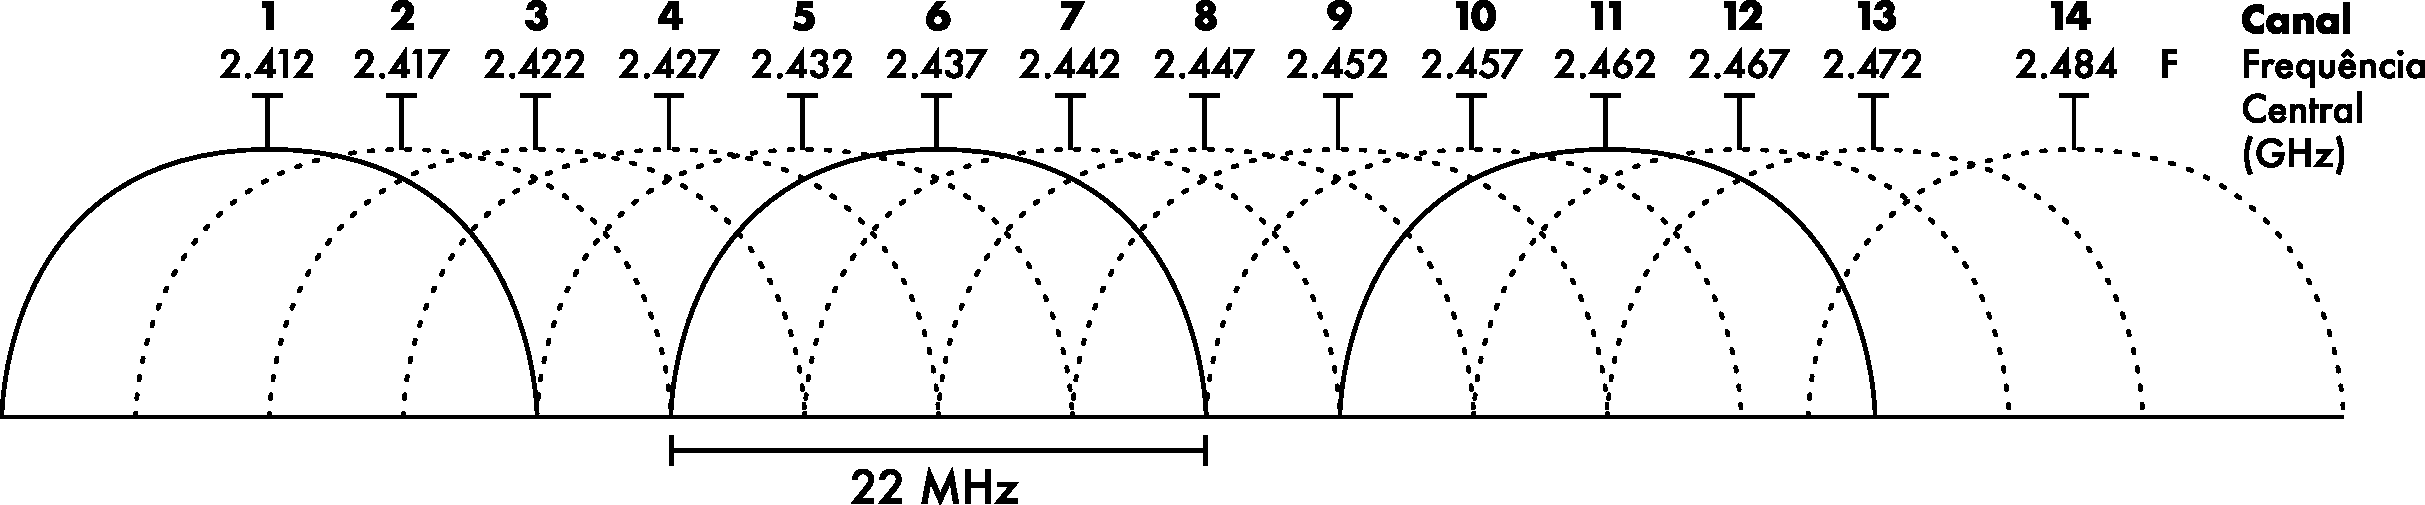
\includegraphics[scale=.36]{figuras/canais_wifi.pdf}
	}{
		\Fonte{\citeonline[p. ~15]{flickenger2008}.}
	}	
\end{figure}

\section{Padrão IEEE 802.11}
\label{sub:padrao-ieee-802-11}

Desde a introdução das redes sem fio como meio de acesso à Internet, o sucesso das mesmas só cresceu, com isso várias empresas procuram formas de padronizar essa tecnologia. O problema é que cada empresa criou seu próprio padrão de rede, o que dificultava a compatibilidade entre equipamentos e protocolos.
Entretanto, para que os equipamentos pudessem se comunicar entre si, deveriam usar os mesmos padrões de comunicação. Com o objetivo de garantir a interoperabilidade dos diversos tipos de equipamentos e fabricantes existentes, os membros do IEEE criaram, em 1997, após sete anos de pesquisa e desenvolvimento, o padrão IEEE 802.11, o primeiro a ser desenvolvido por uma instituição independente, o que impulsionou a sua grande aceitação entre as empresas fabricantes de equipamentos \cite{fluminense2010}.

À medida que a tecnologia de redes sem fio evoluiu, o padrão IEEE 802.11 foi expandido de forma a melhorar aspectos da rede, como a taxa de transmissão e a segurança. Estas melhorias foram incorporadas sob a forma de ``emendas'', designadas por letras acrescentadas ao nome do padrão, como, por exemplo, IEEE 802.11a \cite{fluminense2010}. A seguir, algumas das principais ``emendas'' são explicadas com algum detalhe, de acordo com o ano de surgimento.

\subsection{IEEE 802.11b}
\label{subsec:802-11b}

O padrão 802.11b foi o primeiro padrão IEEE 802.11 aprovado a se popularizar em setembro de 1999. Ele opera na faixa entre 2,4 e 2,4835 GHz e tem a possibilidade de estabelecer conexões nas seguintes velocidades de transmissão: 1 Mbps, 2 Mbps, 5.5 Mbps e 11 Mbps \cite{moraes2010,fluminense2010}. Em ambientes fechados, o IEEE 802.11b consegue ter um alcance de cerca de 35 metros, já para locais abertos pode chegar a 140 metros de alcance.

\subsection{IEEE 802.11a}
\label{802-11a}

O padrão 802.11a foi lançado no mesmo ano que o 802.11b e, apesar de oferecer taxas mais altas, não alcançou a mesma popularidade. As taxas adicionais oferecidas pela emenda ``a'' são: 6 Mbps, 9 Mbps, 12 Mbps, 18 Mbps, 24 Mbps, 36 Mbps, 48 Mbps e 54 Mbps.

As frequências utilizadas por este padrão estão entre 5,725 e 5,875 GHz. Nesta faixa de frequência mais alta, o sinal é mais suscetível a perdas de propagação, diminuindo seu alcance em comparação com a faixa utilizada pelo IEEE 802.11b. Em contrapartida, o uso desta frequência pode ser atraente por estar menos sujeita a interferência de outras fontes. Não existe compatibilidade entre o 802.11a e o 802.11b, pois eles operam em duas faixas de frequência distintas \cite{moraes2010,fluminense2010}.

\subsection{IEEE 802.11g}
\label{subsec:802-11g}

O padrão 802.11g, lançado em 2003, pode ser considerado o sucessor do padrão 802.11b, pois opera na mesma faixa de frequência de 2.4 GHz. Dispositivos que implementam o 802.11g costumam ser retrocompatíveis, isto é, implementam também o 802.11b, sendo muitas vezes especificados como dispositivos 802.11b/g. Sua principal vantagem é a possibilidade de operar com taxas de transmissão de até 54 Mbps, como o IEEE 802.11a, e ao mesmo tempo ter o alcance do IEEE 802.11b \cite{moraes2010,fluminense2010}.

\subsection{IEEE 802.11n}
\label{subsec:802-11n}

O desenvolvimento do padrão 802.11n foi iniciado em 2004 e publicado em 2009. Este padrão pode operar nas faixas de 2.4 GHz e 5 GHz, o que o torna compatível com os padrões anteriores. Sua principal característica é o aumento considerável das taxas de transferência de dados através da combinação de múltiplas vias de transmissão (MIMO, do inglês, \textit{Multiple-Input and Multiple-Output}). O padrão 802.11n pode operar com taxas de transmissão de dados de até 600 Mbps em um canal de 40 MHz \cite{moraes2010}.

\subsection{IEEE 802.11ac}
\label{subsec:802-11ac}

O padrão IEEE 802.11ac foi desenvolvido entre 2011 e 2013 e publicado em dezembro de 2013. Pode ser considerado como o sucessor, em termos de taxa de transmissão, do IEEE 802.11n \cite{alecrim2008site}.
A principal vantagem do 802.11ac está em sua velocidade, estimada em até 433 Mbps no modo mais simples. Mas, teoricamente, é possível fazer a rede superar os 6 Gbps em uma configuração que utiliza múltiplas antenas transmissoras (no máximo, oito antenas podem ser utilizadas). Pelo fato dos equipamentos comumente saírem de fábrica com três antenas, a taxa máxima de transmissão é de aproximadamente 1,3 Gbps \cite{alecrim2008site}.

O 802.11ac trabalha na frequência de 5 GHz, sendo que, dentro desta faixa, cada canal pode ter, por padrão, largura de 80 MHz ou 160 MHz como opcional. Além disso, o 802.11ac possui técnicas de modulação avançadas. Precisamente, o padrão trabalha com a técnica MU-MIMO (do inglês, \textit{Multi-User} MIMO), que permite que sejam transferidos e recebidos dados simultaneamente para todos os terminais, o que resulta em uma melhoria nas velocidades de transferência na mesma frequência de operação \cite{alecrim2008site}.

\subsection{IEEE 802.11ax}
\label{subsec:802-11ax}

O padrão 802.11ax, chamado Wi-Fi 6, um nome mais simples e comercial atribuído pela Wi-Fi Alliance, é o sucessor do 802.11ac. Até momento deste trabalho o Wi-Fi 6 encontra-se em processo de desenvolvimento. Entretanto, já existe fabricantes trabalhando em novos equipamentos compatíveis com o novo padrão de rede sem fio \cite{plaza2018site}.

Com o IEEE 802.11ax a previsão é que os equipamentos consigam operar com a velocidade máxima de 14 Gbps, enquanto na prática a transmissão estará próxima dos 11 Gbps. Diferentemente do 802.11ac que opera apenas na banda de 5 GHz, o Wi-Fi 6 é \textit{dual band} (opera em 2.4 GHz e 5 GHz). Outras promessas são um consumo de energia menor para os dispositivos conectados e uma maior capacidade em manter um bom alcance mesmo com a presença de barreiras, como paredes, que acabam atrapalhando a propagação do sinal pelo ambiente \cite{plaza2018site}.

A visão resumida dos padrões IEEE 802.11 apresentados anteriormente é mostrada na \autoref{tab:resumo-ieee-802-11}.

\begin{table}[H]
	\Caption{\label{tab:resumo-ieee-802-11}Resumo dos padrões IEEE 802.11.}%
	\IBGEtab{}{%
		\begin{tabular}{lccc}
			\toprule
			\multicolumn{1}{c}{Padrão} & \multicolumn{1}{c}{Ano} &  \multicolumn{1}{c}{Banda de Frequência} &  \multicolumn{1}{c}{\textit{Throughput} Máximo (Proposto)} \\
			\toprule %\midrule
			IEEE 802.11b & 1999 & 2.4 GHZ & 11 Mbps \\
			
			IEEE 802.11a & 1999 & 2.4 GHz & 54 Mbps \\
			
			IEEE 802.11g & 2003 & 5 GHz & 54 Mbps \\
			
			IEEE 802.11n & 2009 & 2.4 GHz/5 GHz & 600 Mbps \\
			
			IEEE 802.11ac & 2013 & 5 GHz & 6 Gbps \\
			
			IEEE 802.11ax & Em desenvolvimento & 2.4 GHz/5 GHz & 14 Gbps \\
			\bottomrule
		\end{tabular}%
	}{%
		\Fonte{Adaptado de \citeonline{kar2018ieee}.}%
		%\citeonline[p. ~465]{lott2001ieee}; \apudonline[p.~73]{lott2001ieee}{geier2002}
		\Nota{{\textit{Throughput}, em português, significa taxa de transferência.}}
	}%
\end{table}

\section{Planejamento/Avaliação de Redes Wi-Fi}
\label{sec:alanejamento-avaliação-de-redes-wifi}

Caso surja a necessidade de se planejar a conexão de dispositivos em escritório, residência ou \textit{campus} em uma rede, a implantação da tecnologia Wi-Fi é a solução mais fácil e rápida. A implantação adequada dos componentes básicos (pontos de acesso, cabos e conectores) e a sintonia entre eles é o principal requisito para uma comunicação eficiente e rápida entre os terminais \cite{kar2018ieee}. Para obter um desempenho otimizado de uma LAN sem fio Wi-Fi, é essencial realizar o \textit{site survey} e o planejamento de radiofrequência antes da implantação.

Porém, é importante salientar que uma rede sem fio jamais chega ao mesmo nível de performance da rede cabeada tradicional \cite{moraes2010}. Também é importante considerar que o meio não guiado e a frequência são compartilhados: quanto mais estações conectadas, menor o desempenho final da rede.

\subsection{Site Survey}
\label{subsec:site-survey}

Um procedimento muito importante para o projeto de uma rede sem fio é a utilização de uma metodologia chamada \textit{site survey} (em português, pesquisa do local). Essa metodologia consiste na inspeção técnica minuciosa do local onde será instalada a nova rede, na avaliação dos resultados obtidos da infraestrutura existente ou na identificação e solução dos problemas de um sistema já em funcionamento \cite{pinheiro2004site}.

O \textit{site survey} é uma ferramenta indispensável para detectar e ultrapassar problemas de performance após a implantação de uma nova infraestrutura ou ampliação da rede existente. Durante a inspeção do local, devem ser levantados dados técnicos das condições arquitetônicas do local, que inclui verificar a existência ou não de obstáculos que possam dificultar a distribuição do cabeamento, o posicionamento de equipamentos, a segurança do sistema, etc. \cite{moraes2010,pinheiro2004site}.

No caso específico das redes Wi-Fi, além das condições arquitetônicas do local, a inspeção deve contemplar a análise de possíveis fontes de interferência de radiofrequência, níveis e condições de propagação do sinal, área de cobertura (ou sem cobertura), servindo como fonte adicional de informação para o projeto de posicionamento dos pontos de acesso \cite{pinheiro2004site}. 

Os dados obtidos no \textit{site survey} são usados para estimar o orçamento de recursos técnicos, como requisitos de \textit{hardware}, largura de banda e fontes de energia.
Em seguida, no planejamento de radiofrequência (RF) ajustes finais são feitos na rede para obter um desempenho otimizado em seus parâmetros mais importantes, como:

\begin{compactitem}
\item Capacidade de cobertura: quando existe um grande número de pontos de acesso implantados na mesma área, é iminente o surgimento de interferência originadas das outras redes e de canal adjacente. O planejamento de capacidade é essencial para a implantação de LANs sem fio em grandes áreas como \textit{campus} universitários, aeroportos, \textit{shoppings}, etc. \cite{kar2018ieee}.
  
\item Distribuição da largura de banda: aplicações diferentes tem exigência de largura de banda diferente. O requisito típico de largura de banda para navegação na Web é de 500 kbps, enquanto um processo de videoconferência pode precisar de 2 a 4 Mbps \cite{kar2018ieee}. Uma vez que tais requisitos sejam conhecidos, é possível estimar a largura de banda total necessária para a área de cobertura completa. Portanto, é calculado a necessidade total de largura de banda e sua distribuição em diferentes células de acordo com a demanda exigida pelos clientes da rede \cite{kar2018ieee}.
\end{compactitem}

Por fim, na implantação, é feito o processo de instalação e configuração dos pontos de acesso, fontes de alimentação, cabos, conectores, etc. Uma pesquisa ativa de pós-implantação pode ser realizada para detectar falhas de cobertura e falhas de largura de banda no sistema \cite{kar2018ieee}. A sequência completa de etapas do \textit{site survey} em redes \textit{wireless} está ilustrada pelo fluxograma da \autoref{fig:fluxograma-site-survey}.

\begin{figure}[H]
	\centering
	\Caption{\label{fig:fluxograma-site-survey}Fluxograma para o processo completo do \textit{Site Survey}.}	
	\UECEfig{}{
		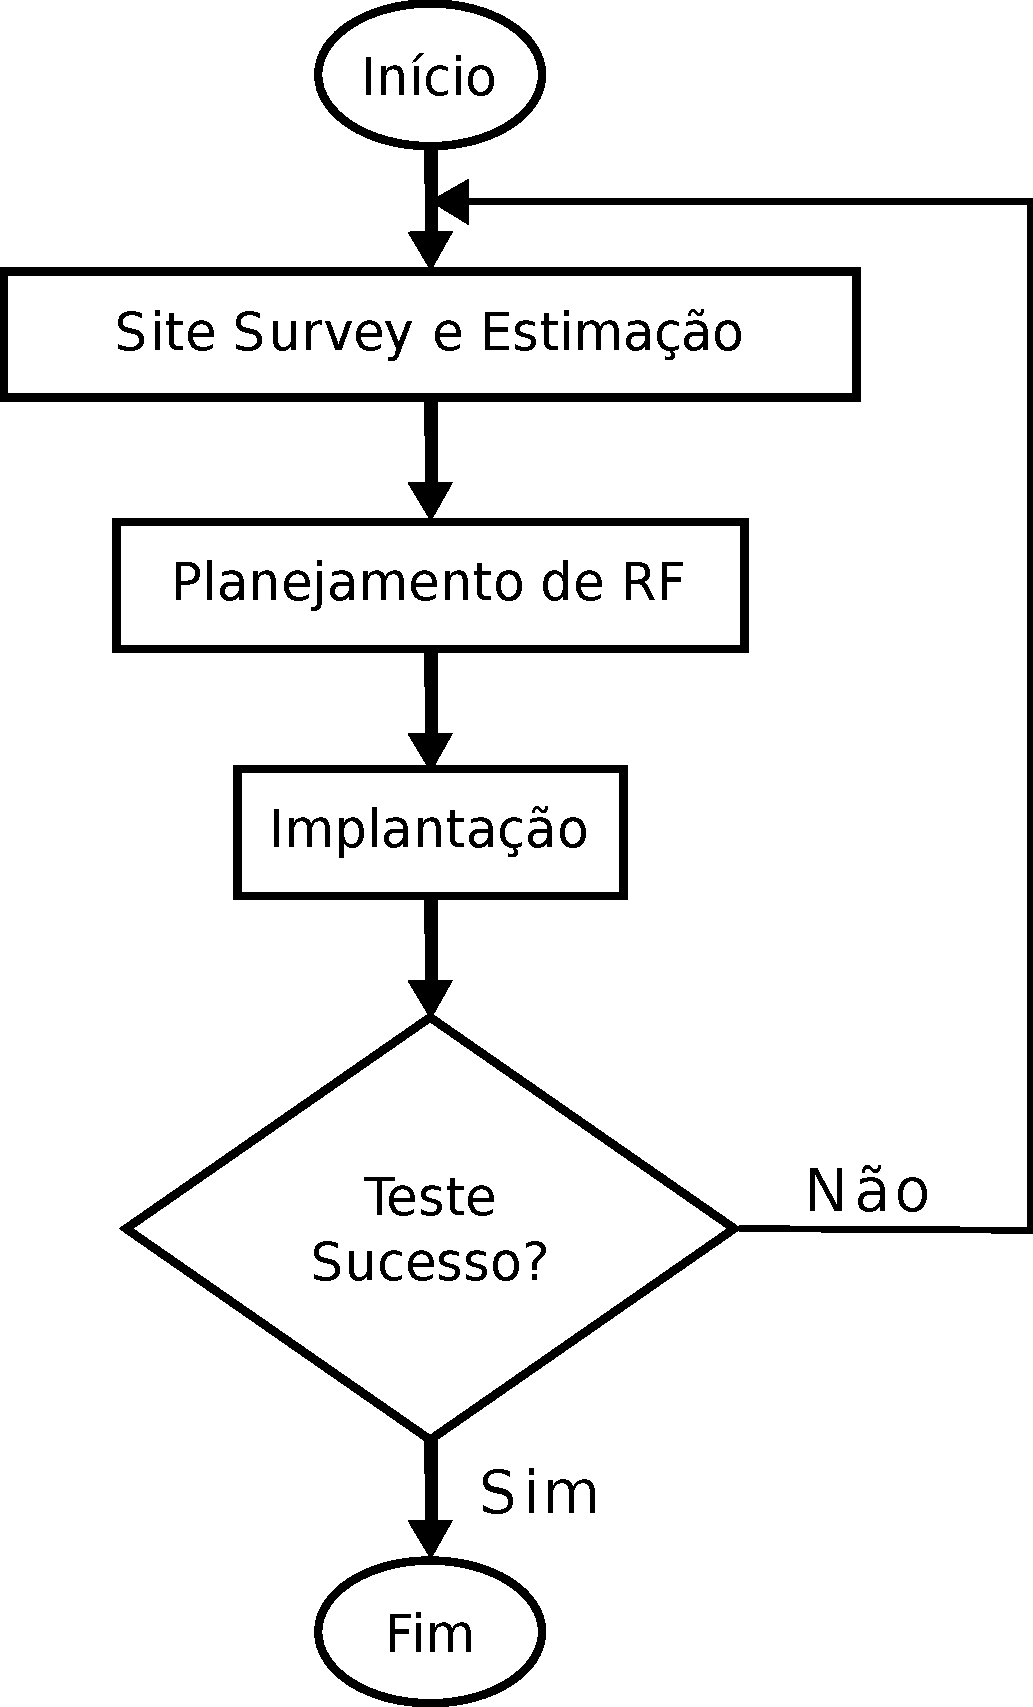
\includegraphics[scale=.38]{figuras/fluxograma-site-survey.pdf}
	}{
		\Fonte{Adaptado de \citeonline{kar2018ieee}.}
	}	
\end{figure}

O principal objetivo de um \textit{site survey} é assegurar que o número, localização e configuração dos pontos de acesso forneçam as funcionalidades requeridas e propiciem um desempenho compatível com a demanda exigida ou com o investimento definido no projeto \cite{pinheiro2004site}. Isso possibilita que todas as estações desfrutem de qualidade nas conexões, tendo total acesso aos serviços disponíveis na rede.

O problema encontrado com maior frequência em redes sem fio é a degradação do sinal devido aos múltiplos caminhos de propagação (multipercurso), causado por reflexões das ondas de rádio em objetos. Portanto, as antenas dos pontos de acesso devem estar dispostas longe de superfícies refletoras, a fim de diminuir as perdas causadas por esse fenômeno \cite{kar2018ieee}.

O processo de pesquisa do local pode ser executado manualmente ou usando um \textit{software} dedicado. A pesquisa manual consiste essencialmente de uma avaliação baseada em \textit{hardware} posteriormente a implantação da rede, enquanto a pesquisa preditiva do local, além da pesquisa em si, inclui o planejamento baseado em simulação computacional \cite{kar2018ieee}.

É possível classificar o \textit{site survey} para redes sem fio em duas categorias dependendo do tipo de ambiente: \textit{indoor} ou \textit{outdoor}.

\textit{Site survey indoor}: consiste em realizar a inspeção buscando interferências, localização e número de pontos de acesso. O equipamento utilizado é basicamente um \textit{notebook} provido de um \textit{software} dedicado instalado e configurado. Esse tipo de inspeção fornece gráficos de intensidade de sinais (mapa de calor), o que torna a análise da cobertura mais precisa e clara. Em prédios, a inspeção pode ser executada em apenas um andar ou em múltiplos andares \apud[p.~73]{rodrigues2007}{geier2002}.

\textit{Site survey outdoor}: consiste em realizar a inspeção de redes \textit{wireless} em uma escala muito maior que a existente na modalidade \textit{indoor}. Além da localização e posição de pontos de acesso e das antenas de transmissão de grande porte, verifica-se a existência de linha de visada direta ou não com o fonte transmissora \cite{pinheiro2004site}. Essa modalidade de inspeção produz mapas de calor com maior complexidade de análise, devido às dimensões do terreno, da variabilidade do relevo e da grande quantidade de fontes de interferência \apud[p.~73]{rodrigues2007}{geier2002}.

\subsubsection{Softwares de Site Survey}
\label{subsubsec:softwares-site-survey}

Implantar uma rede Wi-Fi que cubra uma grande área e com um sinal forte não é uma tarefa fácil. Devido à interferência causada por outras redes Wi-Fi e à presença de grandes obstáculos tais como paredes e mobília, muitas redes Wi-Fi são castigadas por quedas frequentes da conexão, velocidades baixas, e a presença de zonas sem cobertura de sinal (áreas de sombra).

No entanto, é possível otimizar o desempenho de uma rede Wi-Fi com a ajuda de uma ferramenta de \textit{software} específica que gere, por exemplo, um mapa de calor, que consiste em um mapa da cobertura e força do sinal \textit{wireless} baseado na representação real do local de interesse. No mapa de calor é possível identificar, de acordo com a colorização dos setores, onde os nível de potência do sinal é mais forte ou mesmo inexiste, contribuindo para eventuais alterações na infraestrutura da rede.

\subsubsubsection{NetSpot}
\label{subsubsubsec:netspot}

Disponível para o sistema operacional MacOS e Windows, NetSpot é a ferramenta de \textit{software} de \textit{site survey} paga projetada para ser utilizada tanto por profissionais quanto por usuários domésticos para a análise e levantamento de redes Wi-Fi e pode ser usado inspecionar qualquer padrão de rede 802.11 já implementado \cite{Netspot2019}. Dispõe de uma interface gráfica intuitiva, facilitando sua utilização.

Com o NetSpot é possível criar, na janela \textit{survey}, um mapa de calor a partir do \textit{upload} do arquivo que representa o local real (\autoref{fig:netspot}). Em seguida, basta o deslocamento de um local a outro para a coleta dos dados e aguardar a construção automática do gráfico com a intensidade do sinal de cada ponto. Além disso, o NetSpot possui a capacidade de analisador Wi-Fi, coletando informações detalhadas sobre as redes \textit{wireless} próximas, incluindo o seu nome (SSID, do inglês, \textit{Service Set Identifier}), o tipo de segurança que usam, em qual canal transmitem, e a potência do sinal, entre outras características \cite{Netspot2019}.

\begin{figure}[H]
	\centering
	\Caption{\label{fig:netspot}Tela de \textit{survey} do NetSpot.}	
	\UECEfig{}{
		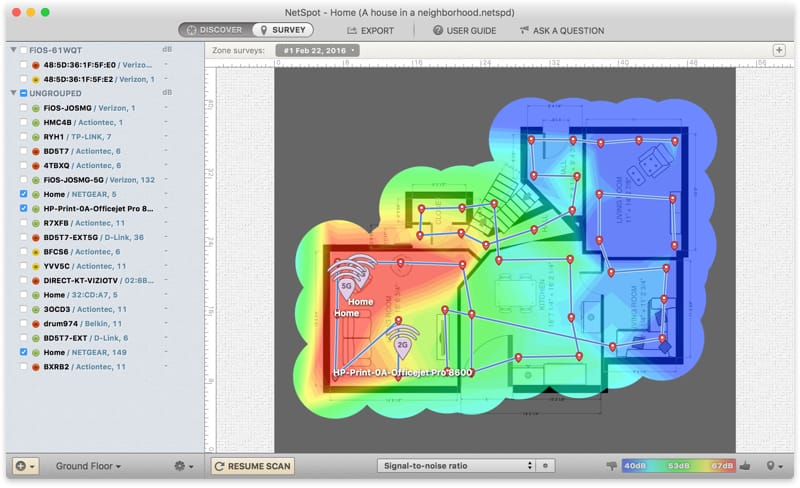
\includegraphics[scale=.48]{figuras/tela_netspot.jpg}
	}{
		\Fonte{\citeonline{Netspot2019}.}
	}
\end{figure}

\subsubsubsection{Ekahau HeatMapper}
\label{subsubsubsec:ekahau}

Ekahau HeatMapper é um \textit{software} de inspeção objetivo, com suporte para os padrões 802.11a/b/g/n e uma interface de usuário simples (\autoref{fig:ekahau}). Esta ferramenta, além do mapa de calor, pode descobrir automaticamente todos os pontos de acesso próximos e detectar as suas configurações básicas \cite{Ekahau2019}. O Ekahau HeatMapper pode ser adquirido gratuitamente pelo site do desenvolvedor e funciona em qualquer \textit{notebook} com Windows ou computador \textit{desktop} com um adaptador Wi-Fi.

\begin{figure}[H]
	\centering
	\Caption{\label{fig:ekahau}Tela de principal do Ekahau HeatMapper.}	
	\UECEfig{}{
		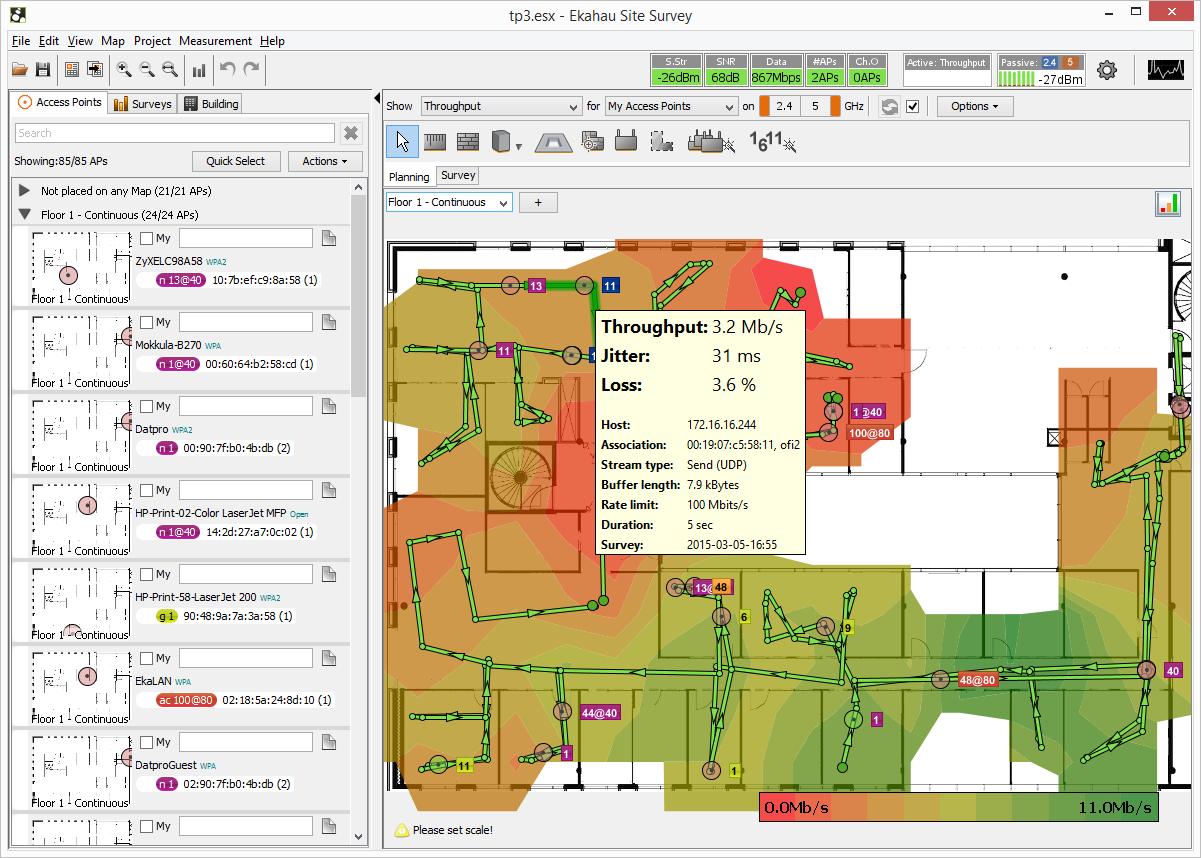
\includegraphics[scale=.38]{figuras/Ekahau-HeatMapper.png}
	}{
		\Fonte{\citeonline{Ekahau2019}.}
	}
\end{figure}

\subsubsubsection{Acrylic Wi-Fi Heatmaps}
\label{subsubsubsec:acrylic-wifi-heatmaps}

O Acrylic Wi-Fi Heatmaps consiste de uma ferramenta avançada de análise de rede sem fio para obter uma visão detalhada do cenário \textit{wireless} ao redor. O Acrylic Wi-Fi Heatmaps pode analisar tanto o espectro de frequência de 2.4 GHz quanto o de 5 GHz e gerar mapas de calor detalhados e relatórios em uma variedade de formatos de arquivo comum (Word, CSV, KMZ) \cite{Netspot2019}. 

O gráfico de cobertura  de sinal gerado por esta ferramenta de \textit{software} (ilustrado na \autoref{fig:acrylic}) pode ser baseado tanto em mapas online, bem como em mapas importados pelo usuário. O Acrylic Wi-Fi Heatmaps torna possível editar os mapas gerados, que é algo que os profissionais podem apreciar. O \textit{software} está disponível gratuitamente para experimentação limitada, tendo a opção de compra com todas as funcionalidades liberadas.

\begin{figure}[H]
	\centering
	\Caption{\label{fig:acrylic}Tela de geração de mapas de calor do Acrylic Wi-Fi Heatmaps.}	
	\UECEfig{}{
		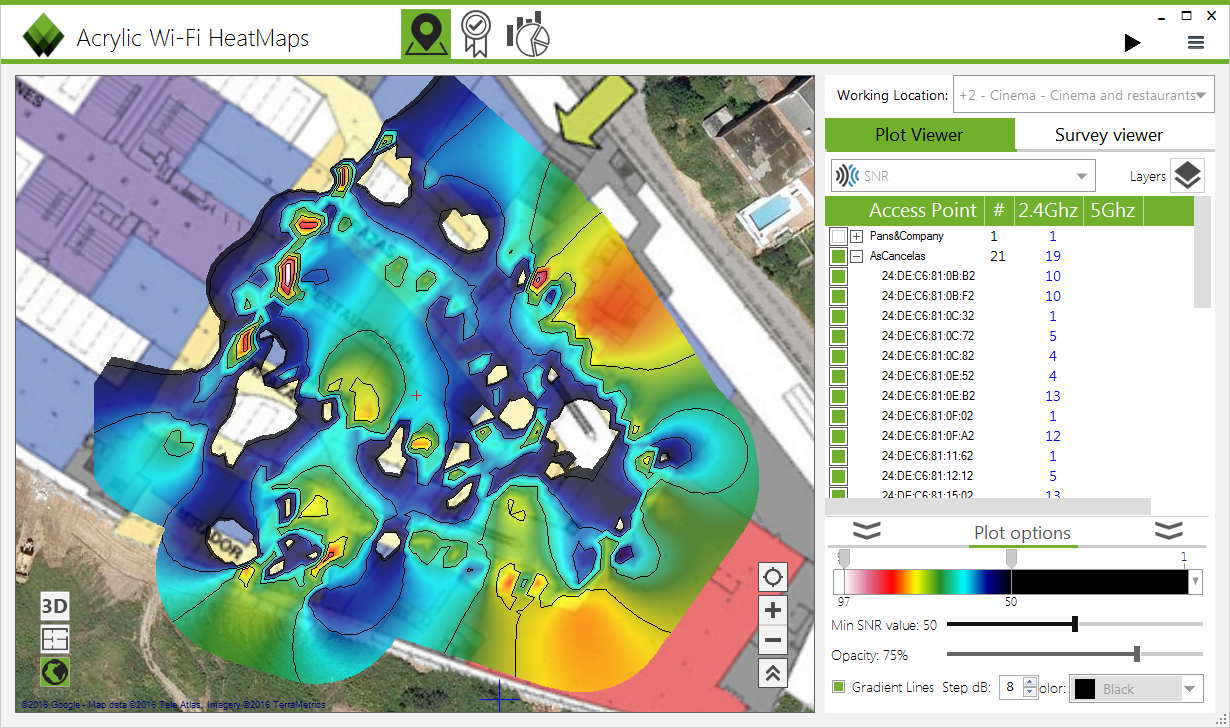
\includegraphics[scale=.28]{figuras/Acrylic-Wi-Fi-Heatmaps.png}
	}{
		\Fonte{\citeonline{Netspot2019}.}
	}
\end{figure}

\subsubsubsection{VisiWave Site Survey}
\label{subsubsubsec:visiwave}

O VisiWave Site Survey destina-se especialmente a inspeções de larga escala, como pode ser visto na \autoref{fig:visiwave}, sendo capaz de fornecer três métodos eficazes para a captura de dados: um ponto de cada vez; caminhadas contínuas pela área de pesquisa e posicionamento GPS (do inglês, \textit{Global Positioning System}) para levantamentos ao ar livre. 

É possível criar relatórios personalizados ou reutilizar modelos de relatórios para visualizar sua cobertura ou visualizar interativamente os dados de cobertura no Google Earth\footnote[5]{Google Earth é um programa de computador desenvolvido e distribuído pela empresa estadunidense do Google cuja função é apresentar um modelo tridimensional do globo terrestre, construído a partir de mosaico de imagens de satélite obtidas de diversas fontes.} \cite{Netspot2019}. O VisiWave Site Survey suporta a maioria dos adaptadores de rede Wi-Fi, e não requer nenhum componente de \textit{hardware} especial para funcionar.
\newpage
\begin{figure}[H]
	\centering
	\Caption{\label{fig:visiwave}Tela de geração de mapas de calor do VisiWave Site Survey.}	
	\UECEfig{}{
		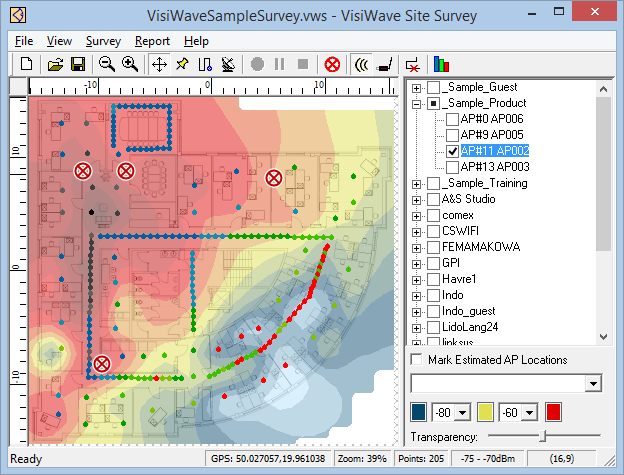
\includegraphics[scale=.64]{figuras/VisiWave-Site-Survey.png}
	}{
		\Fonte{\citeonline{Netspot2019}.}
	}
\end{figure}

\subsubsubsection{AirMagnet Survey PRO}
\label{subsubsubsec:airmagnet-pro}

O AirMagnet Survey PRO pode criar um mapa de calor de leitura fácil para sinal/ruído, taxa de transferência de LAN sem fio, taxas de dados, taxas de repetição e as perdas de pacotes da rede, aliado com uma interface gráfica visualmente rica em opções (\autoref{fig:airmagnet-pro}). Este \textit{software} suporta todos os padrões de rede Wi-Fi e possui suporte a um grande número de recursos \cite{Netspot2019}.

\begin{figure}[H]
	\centering
	\Caption{\label{fig:airmagnet-pro}Tela de geração de mapas de calor do AirMagnet Survey PRO.}	
	\UECEfig{}{
		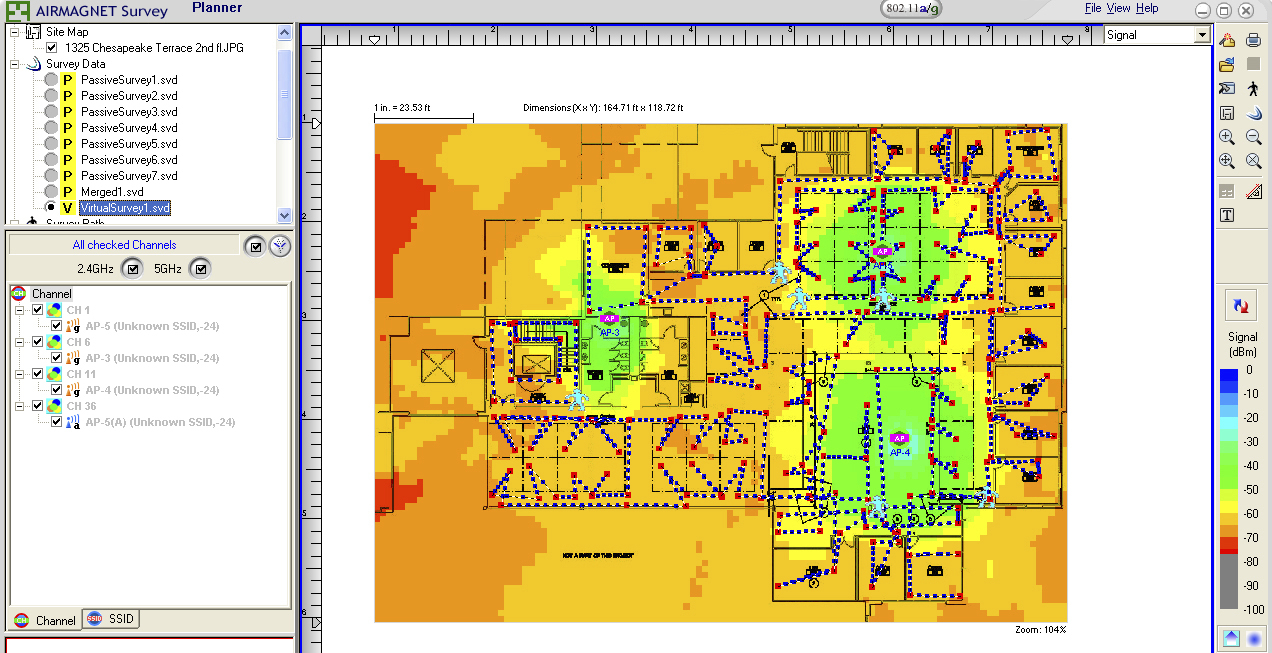
\includegraphics[scale=.38]{figuras/AirMagnet-Survey-PRO.jpg}
	}{
		\Fonte{\citeonline{Netspot2019}.}
	}
\end{figure}

\subsubsubsection{Xirrus Wi-Fi Inspector}
\label{subsubsubsec:xirrus-wifi}

O Xirrus Wi-Fi Inspector é um \textit{software} de análise direcionado principalmente para usuários que frequentemente acessam a Internet utilizando computadores portáteis e desejam um método fácil de encontrar redes Wi-Fi, disponível em versão grátis e paga, e com uma interface gráfica amigável e simples (\autoref{fig:xirrus-wifi}). Além de mostrar o SSID, velocidade e o tipo de segurança de cada rede disponível, o programa ainda indica a distância de cada ponto de acesso em relação ao usuário e permite realizar uma série de testes que verificam tanto a velocidade da conexão quanto sua estabilidade.

\begin{figure}[H]
	\centering
	\Caption{\label{fig:xirrus-wifi}Tela principal do Xirrus Wi-Fi Inspector.}	
	\UECEfig{}{
		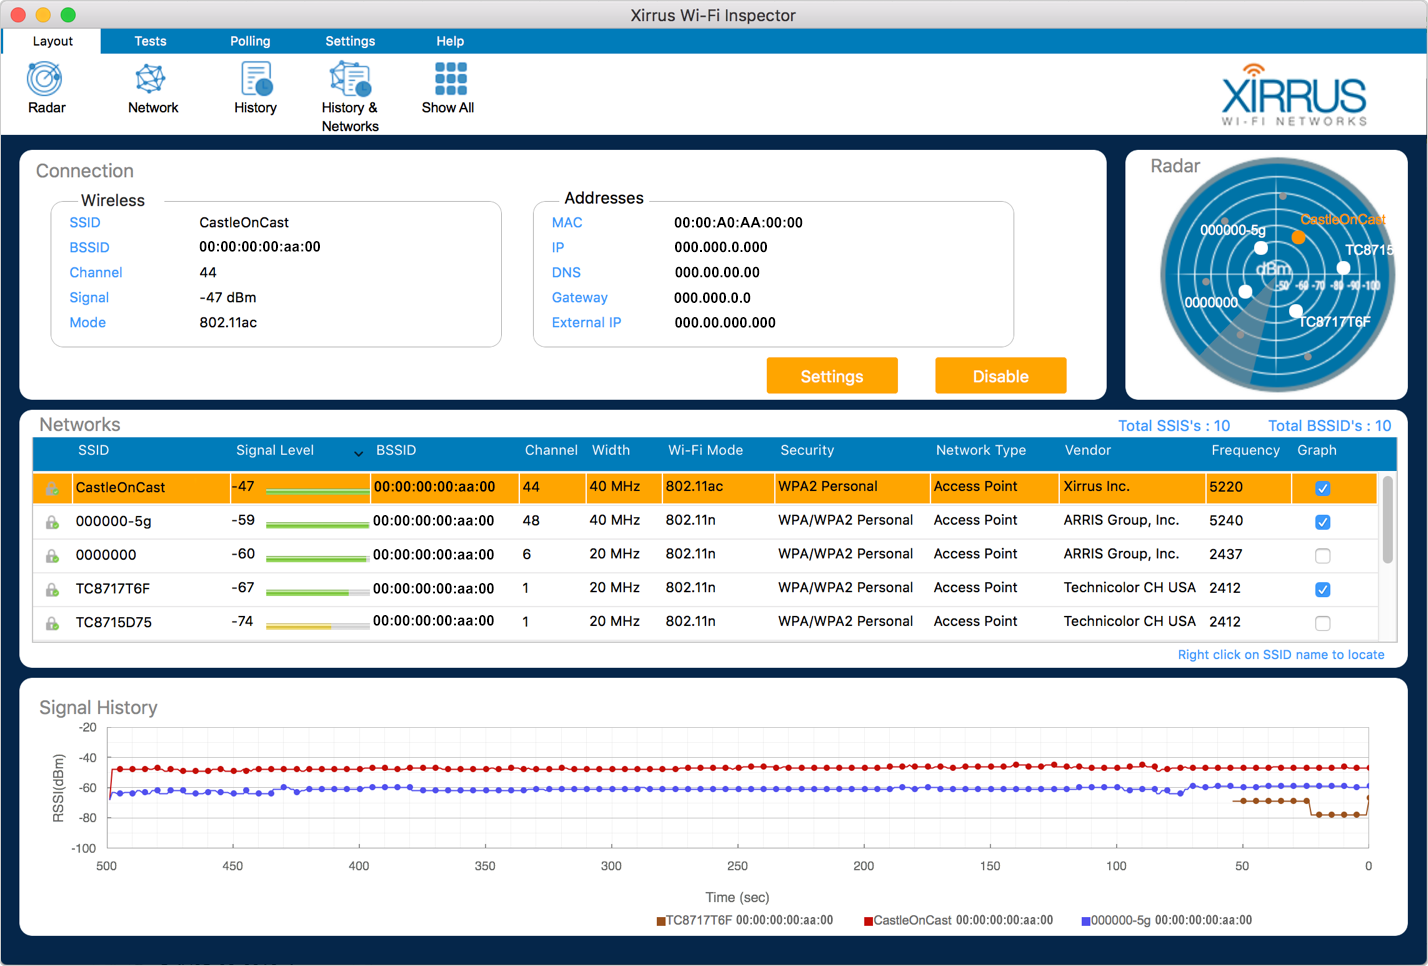
\includegraphics[scale=.27]{figuras/xirrus.png}
	}{
		\Fonte{\citeonline{Xirrus}.}
	}
\end{figure}